%%%%%%%%%%%%%%%%%%%%%%%%%%%%%%%%%%%%%%%%%%%%%%%%%%%%%%%%%%%%%%%%%%
%%
%%                Proceedings of the annual meeting 
%%               of the French Astronomical Society  
%%      Societe Francaise d'Astronomie et d'Astrophysique  (SF2A)
%% 
%%%%%%%%%%%%%%%%%%%%%%%%%%%%%%%%%%%%%%%%%%%%%%%%%%%%%%%%%%%%%%%%%%
%%
%% These proceedings are published electronically in English.
%%
%% The proceedings must be prepared using the present template.
%% Please follow rigorously the instructions. 
%%
%% The recommended number of pages is:
%%   * Review -> 6 pages
%%   * Oral contribution -> 4 pages
%%   * Poster -> 2 pages
%% 
%% All your files must named as follows:
%%     surname.tex, surname.bib, surname_fig1.pdf, surname_fig2.pdf...
%%
%% And if you have several contributions:
%%     surname1.tex, surname2.tex ... etc
%%     surname1_fig1.pdf, surname2_fig1.pdf, ... etc
%%
%% Please provide only PDF figures 
%% To convert figures from eps to pdf, you may use epstopdf
%%
%% Once completed, please send your proceeding as a single tar.gz (surname_SXX.tar.gz)
%% file at proceedings@sf2a.eu before September 29th 2023
%% Please mention the subject: "Proceedings SF2A 2023". Also include the name/number of the session
%% the contribution belongs to as well as the type of your contribution (review, oral cont., poster)
%%
%% Please send on tar archive per contribution! If you have more than one contribution
%% in a given session appen a suffix (a,b,c) to the session number.
%% 
%% Thank you !
%%
%%%%%%%%%%%%%%%%%%%%%%%%%%%%%%%%%%%%%%%%%%%%%%%%%%%%%%%%%%%%%%%%%%
\documentclass{sf2a-conf2023}
\usepackage{graphicx}
\usepackage{hyperref}
\usepackage[]{natbib}  
\usepackage{epstopdf}
\renewcommand{\thefootnote}{\fnsymbol{footnote}}
\def\BibTeX{{\rm B\kern-.05em{\sc i\kern-.025em b}\kern-.08em
    T\kern-.1667em\lower.7ex\hbox{E}\kern-.125emX}}
\bibpunct{(}{)}{;}{a}{}{,}  %%%%%%%%%%%%%  A&A bibliography style
%%-----------------------------------------------------------------
%%         your macros below:
%%
\newcommand{\kms}{{\mathrm{km~s^{-1}}}}
\newcommand{\kpc}{{\mathrm{kpc}}}
%%-----------------------------------------------------------------
%%
%%%%%%%%%%%%%%%--BODY--%%%%%%%%%%%%%%%%%%

\begin{document}

\TitreGlobal{SF2A 2023}

%%-----------------------------------------------------------------
%%      the top matter
%%

\title{This is the title of the paper}

\runningtitle{Short title here}

\author{A. Author1}\address{Timberland Observatory, 34560 City, Neverland}

\author{J.-P. Author2}\address{Institute XYZ, 1299 City, OtherLand}

%% IF Author3 has the same affiliation than Author1:
%\author{C.\,E. Author3$^1$}

%% IF Author3 has its own affiliation:
%\author{C.\,E. Author3}\address{Dept. of Chess, University of Games, 35101 Las Vegas, Monaco} 

%% IF Author3 has two affiliations, the one of Author1 and a second one:
\author{C.\,E. Author3$^{1,}$}\address{Dept. of Chess, University of Games, 35101 Las Vegas, Monaco} 


%% Keep this line, even if the page will be settled afterwards.
\setcounter{page}{237}



%%-----------------------------------------------------------------

\maketitle

%%-----------------------------------------------------------------
%%        The abstract
%% 
%%  Warning!  within the abstract:
%%  - do not use macros. 
%%  - do not use commands like: \cite, \citet, \citep ... etc.

\begin{abstract}
This is the abstract. This is the abstract. This is the abstract.
\end{abstract}


%% Insert the keywords (to appear in the ADS indexing)
%% Keywords must be separated by a comma
\begin{keywords}
subject, verb, noun, apostrophe
\end{keywords}

%%-----------------------------------------------------------------


\section{Introduction}
%%---------------------
  Enter here the text of your introduction.
  
\section{My first section}
%%-------------------------


\subsection{ Literature citations}
%%---------------------------------
 
The following examples illustrate the required style in the main text:
 \cite{Einstein26} showed that $v_h = 1926 \, \kms$ was not a prime number, as
 also found previously \citep{Laurel24}. On the other hand, 
  \citet{1945RvMP...17..120E} followed 
\citet{Kafka24} and found a better approximation to the
distance, yielding $d_o = 22 \, \kpc$ \citep[see also][and references therein]{Bohr26,Curie91,deGaulle96}. 
For frequently cited papers an abbreviated form of citation is
 recommended, e.g. Paper~I, Paper~II.

The format for references is the one adopted by A\&A. To set the reference list in the proper format, we encourage you to use \BibTeX~ and the natbib package instead of the standard \verb=\thebibliography= environment.

\subsection{Footnotes}
%%---------------------

These should be kept to a minimum and used as 
usual\footnote{Just like this one.}.


\subsection{Hyperlinks}

Hyperlinks can be introduced as follows: \url{http://www.sf2a.eu/}.

\subsection{Figures}
%%-------------------

Please use files in the PDF format, as shown in Fig.~\ref{author1:fig1}. Figures in eps format can be converted to pdf with the command epstopdf (used as ``epstopdf file.eps''). Two figures can be joined together as shown in Fig.~\ref{author1:fig2}. In this case, as illustrated in Fig.~\ref{author1:fig2}, 
the caption must follow this format (e.g. boldface fonts for the Left and Right items): \textbf{Left:} text
of the caption for the left panel. \textbf{Right:} text of the caption for the figure on the right hand side. 

%%
%% Example of single figure
%%
\begin{figure}[ht!]
 \centering
 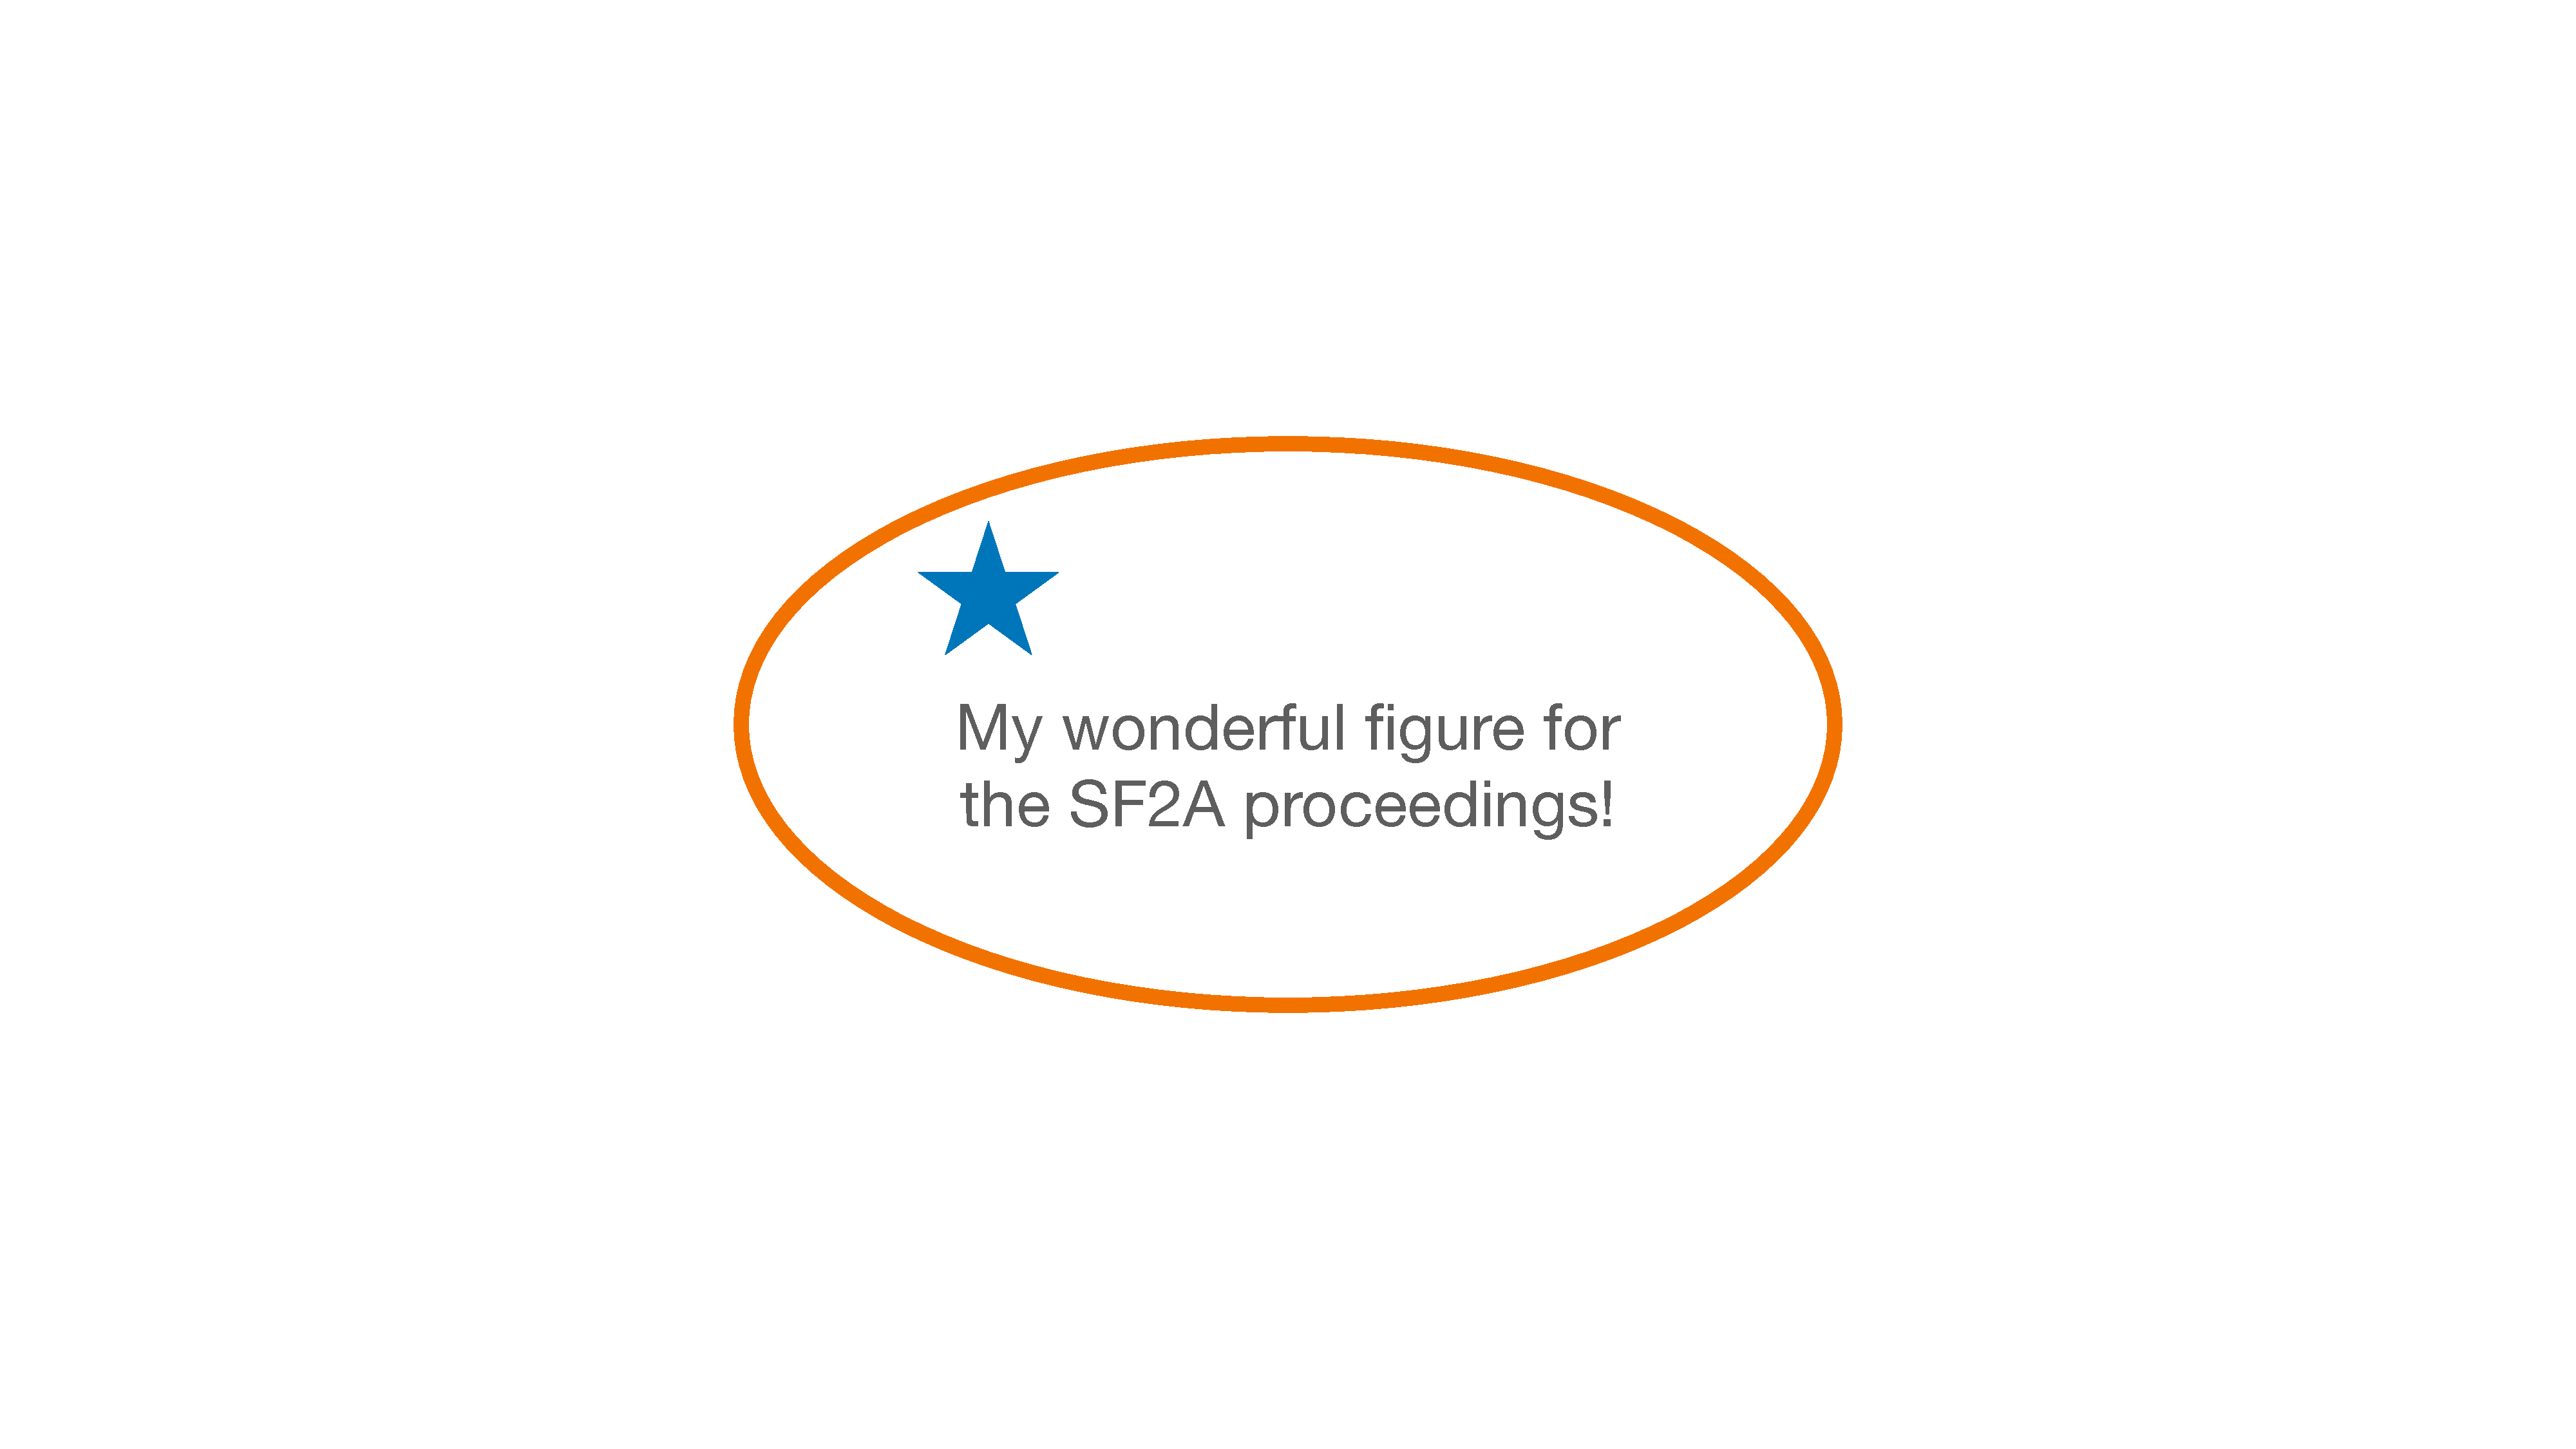
\includegraphics[width=0.8\textwidth,clip]{author_fig1}      
%% Note the ABSENCE of the extension .pdf  !
  \caption{Caption here}
  \label{author1:fig1}
\end{figure}

%%
%% Example of two figures side by side
%%
\begin{figure}[ht!]
 \centering
%% 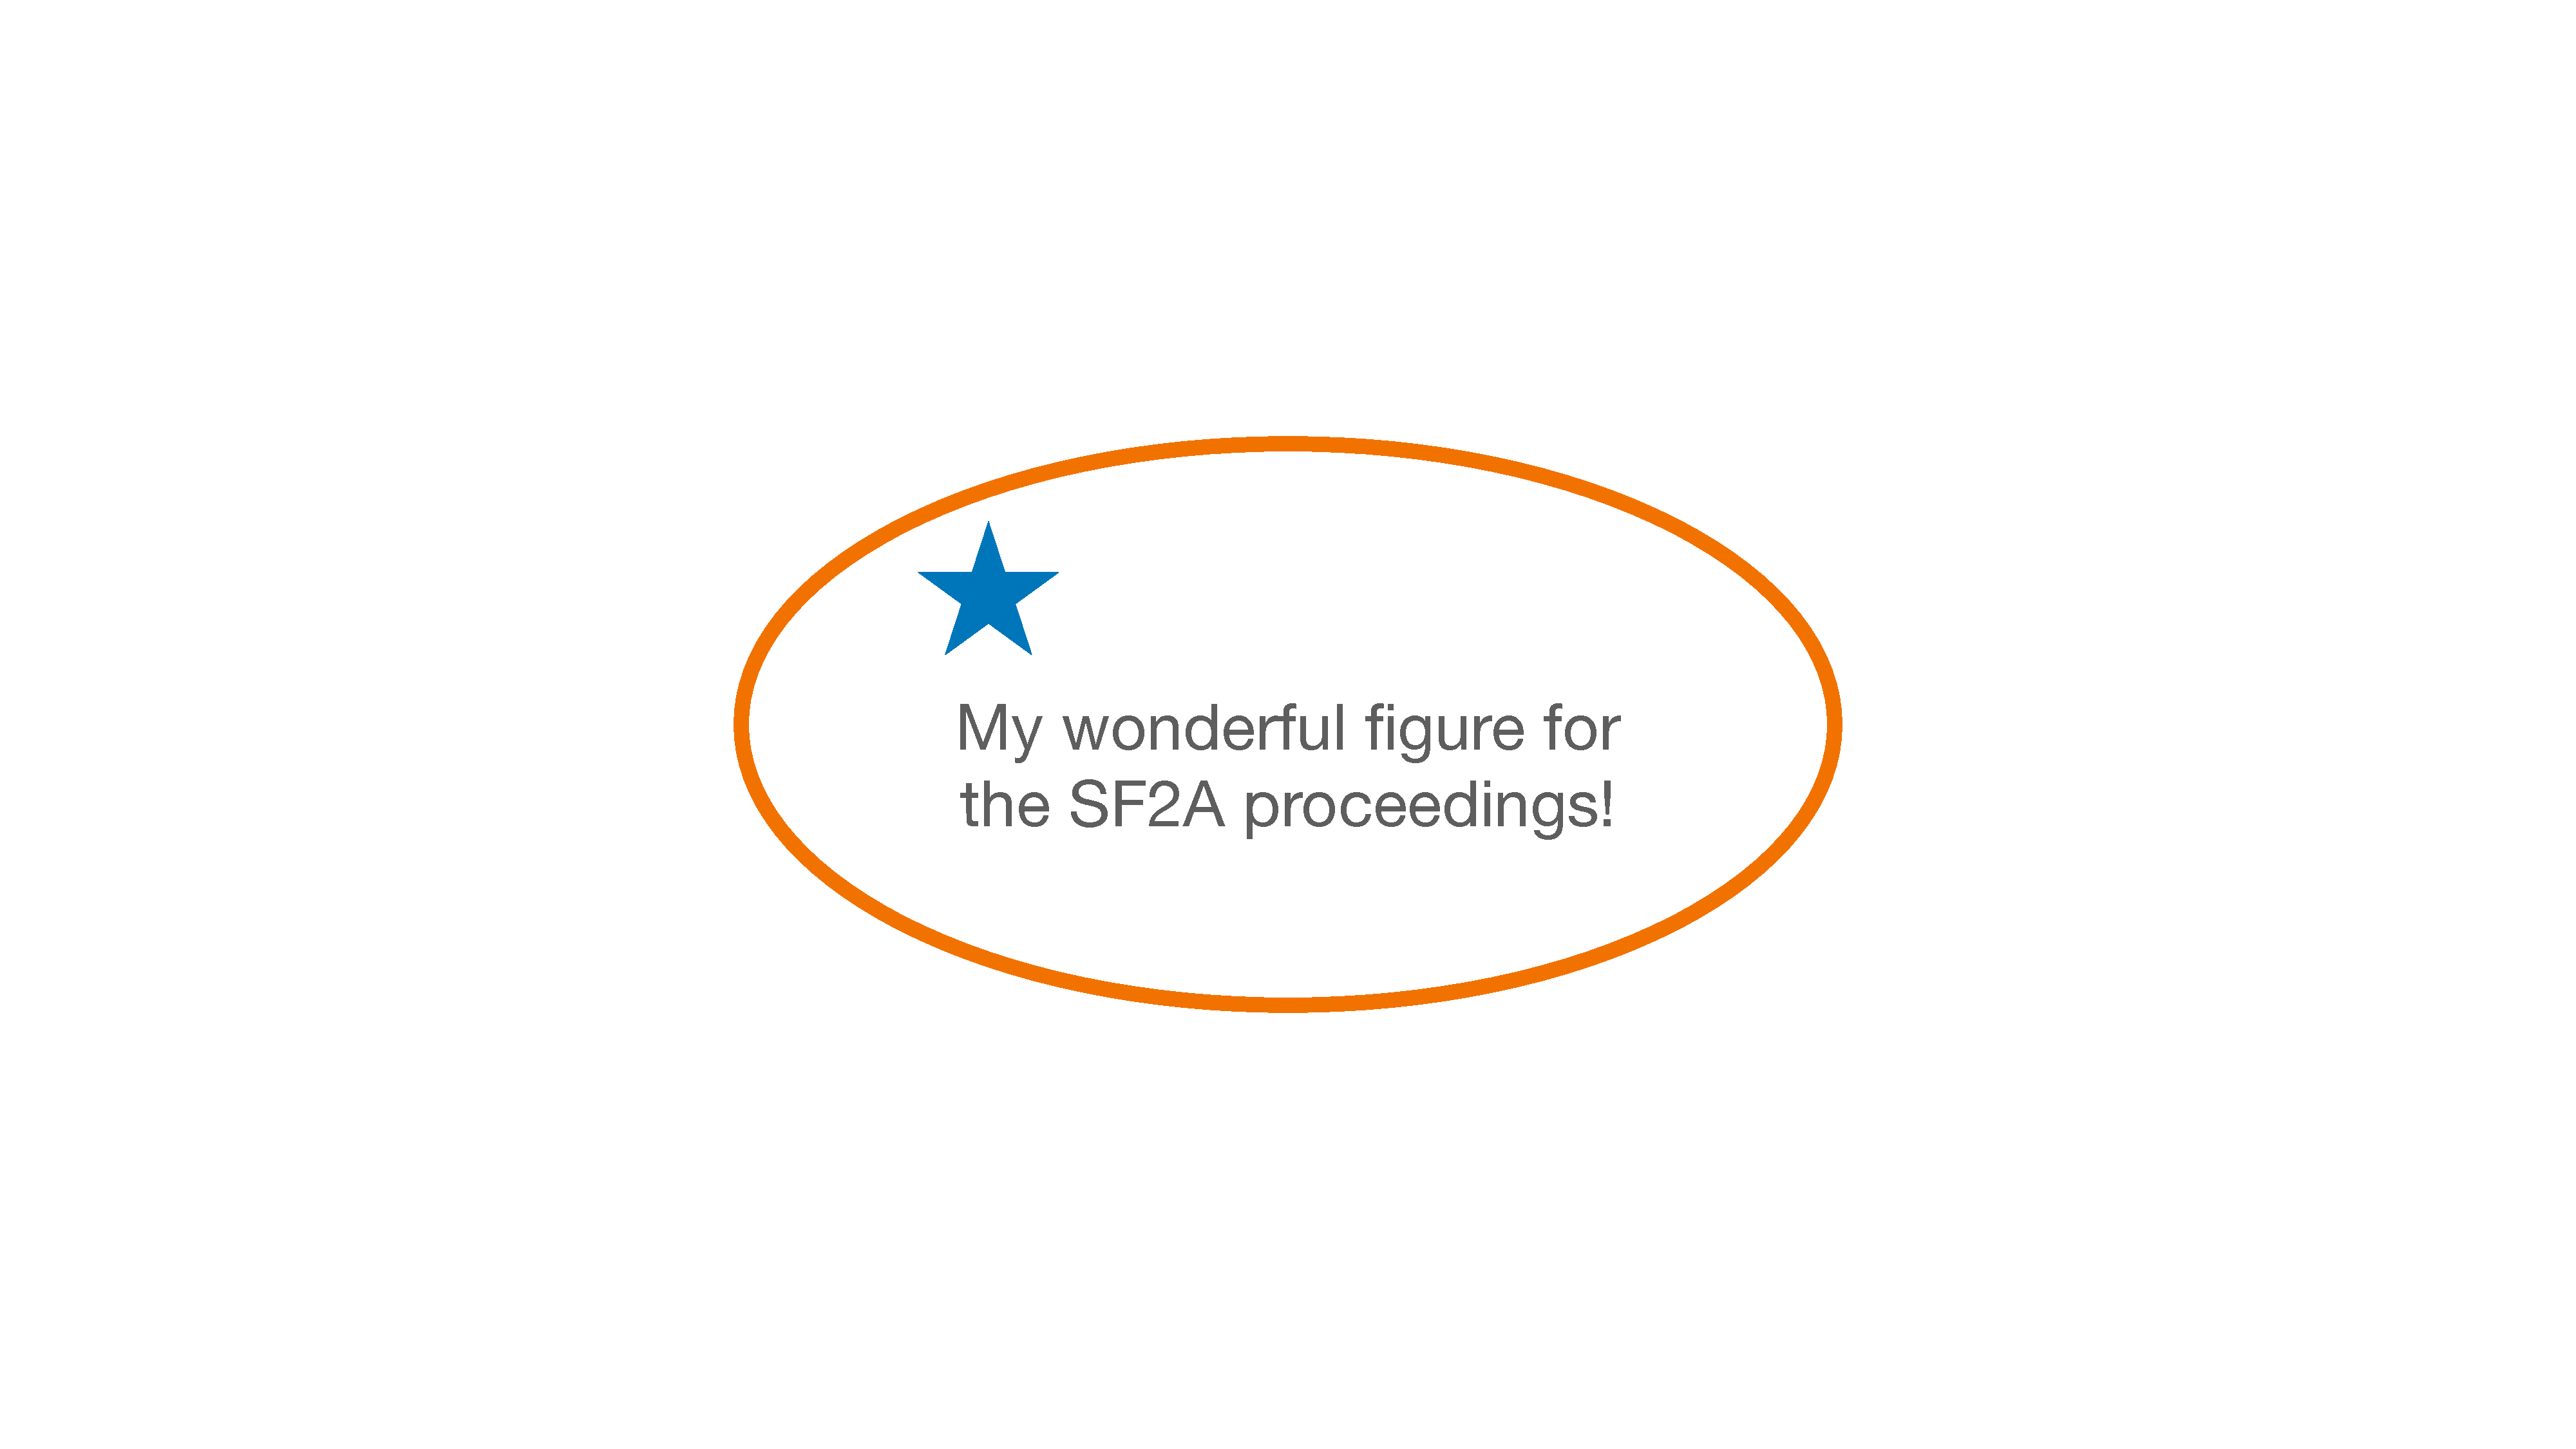
\includegraphics[width=0.48\textwidth,clip]{author_fig1}%      
%% \includegraphics[width=0.48\textwidth,clip]{author_fig2}      
%% Note the ABSENCE of the extension .pdf  !
  \caption{{\bf Left:} Caption of the left panel. {\bf Right:} Caption of the right panel. }
  \label{author1:fig2}
\end{figure}

\section{Conclusions}
%%--------------------

This is the conclusion of the article.

% Optional acknowledgements
% -------------------------
\begin{acknowledgements}
The standard acknowledgement, if required, is : Thank you!
\end{acknowledgements}

%%-----------------------------
%%   Bibliography
%%-----------------------------
%%
%% The reference list should contain all the references cited in the text, ordered alphabetically by surname (with
%% initials following). If there are several references to the same first author, they should be entered according
%% to the following scheme:
%% 1. One author: chronologically
%% 2. Author, one co-author: alphabetically by co-author, then chronologically
%% 3. Author, two or more co-authors: chronologically.
%%
%% Please note that for papers that have more than five authors, only the first three should be given, followed
%% by "et al."
%%
%% The format for references is the one adopted by A&A (see the example below).
%%
%% To set the reference list in the proper A&A format, we encourage you to use BibTEX and the natbib
%% package instead of the standard 'thebibliography' environment.
%%

%\begin{thebibliography}{}
%\bibitem[Bohr et al.(1992)]{Bohr26} Bohr, N., Einstein, A., \& Fermi, E. 1992, MNRAS, 301, 257
%\bibitem[Curie \& Curie(1991)]{Curie91} Curie, M., \& Curie, P. 1991, A\&A, 248, 612
%\bibitem[de Gaulle(1996)]{de Gaulle96} de Gaulle, C. 1996, Solar Phys. (Oxford Univ. Press, Oxford)
%\bibitem[Einstein(1926)]{Einstein26} Einstein, A. 1926, ApJ, 63, 196 (Paper~II) 
%\bibitem[Einstein \& Strauss(1945)]{1945RvMP...17..120E} Einstein, A., 
%\& Strauss, E.G. 1945, Rev. Mod. Phys., 17, 120
%\bibitem[Kafka et al.(1924)]{Kafka24} Kafka, F., Laurel, S., Hardy, O. et al. 1924, A\&A, 248, 612
%\bibitem[Laurel \& Hardy(1994)]{Laurel94} Laurel, S., \& Hardy, O. 1994, Active Driking, in The Evolution
% and Distribution of Beverages, eds. W. Churchill, F. D. Roosevelt, \& A. Capone (Chicago: Bourbon Distilleries Inc.), p. 234 
%\end{thebibliography}

%% The following lines are required when using BibTEX (strongly encouraged!):
\bibliographystyle{aa}  % A&A bibliography style file (aa.bst)
\bibliography{sf2a-template} % your references in file: Yourfile.bib


%
\end{document}
%%%%%%%%%%%%%%%%%%%%%%%%%%%%%%%%%%%%%%%%%%%%%%%%%%%%%%%%%%%%%%%%%%
